%%%%%%%%%%%%%%%%%%%%%%%%%%%%%%%%%%%%%%%%%%%%%%%%%%%%%%%%%%%%%%%%%%%%%%%%%%%%%%%
%                         File: osa-revtex4-1.tex                             %
%                        Date: April 15, 2013                                 %
%                                                                             %
%                              BETA VERSION!                                  %
%                   JOSA A, JOSA B, Applied Optics, Optics Letters            %
%                                                                             %
%            This file requires the substyle file osajnl4-1.rtx,              %
%                   running under REVTeX 4.1 and LaTeX 2e                     %
%                                                                             %
%                   USE THE FOLLOWING REVTeX 4-1 OPTIONS:                     %
% \documentclass[osajnl,twocolumn,showpacs,superscriptaddress,10pt]{revtex4-1}%
%                    %% Use 11pt for Applied Optics                           %
%                                                                             %
%               (c) 2013 The Optical Society of America                       %
%                                                                             %
%%%%%%%%%%%%%%%%%%%%%%%%%%%%%%%%%%%%%%%%%%%%%%%%%%%%%%%%%%%%%%%%%%%%%%%%%%%%%%%

\documentclass[osajnl,twocolumn,showpacs,superscriptaddress,10pt]{revtex4-1} %% use 10pt for Applied Optics
%%\documentclass[osajnl,preprint,showpacs,superscriptaddress,12pt]{revtex4-1} %% use 12pt for preprint option
\usepackage{amsmath,amssymb,graphicx,float,enumerate}
% \usepackage[cache=false]{minted}
\usepackage[utf8]{inputenc}
\graphicspath{ {../images/} }

\usepackage{silence}
\WarningFilter{revtex4-1}{Repair the float}

\begin{document}

\title{Redes y Comunicaciones}

\author{Ulises Jeremias Cornejo Fandos}
\affiliation{13566/7, Licenciatura en Informatica, Facultad de Informatica, UNLP}

\author{Federico Ramón Gasquez}
\affiliation{13598/6, Licenciatura en Informatica, Facultad de Informatica, UNLP}

\author{Lihuel Pablo Amoroso}
\affiliation{13497/2, Analista Programador Universitario, Facultad de Informatica, UNLP}

%%\begin{abstract}
%%\end{abstract}

\maketitle %% required

\onecolumngrid

\section{Ejercicio 1}

\textit{Cuántos intentos de conexiones TCP hay en la captura?} \\

Filtrando los paquetes TCP de la captura dada podemos ver que hay 2 intentos de conexiones.

\section{Ejercicio 2}

\textit{Cuales son la fuente y el destino (IP:port) para c/u?} \\

En el primer intento de conexión se pueden identificar los siguientes fuente y destino.

\begin{itemize}
    \item \textbf{Fuente:} 10.0.1.10:51375
    \item \textbf{Destino:} 10.0.3.10:5001
\end{itemize}

En el segundo intento de conexión, \textit{paquetes 7, 8 y 9}, se pueden identificar los siguientes fuente y destino.

\begin{itemize}
    \item \textbf{Fuente:} 10.0.1.10:51376
    \item \textbf{Destino:} 10.0.3.10:5001
\end{itemize}

\section{Ejercicio 3}

\textit{Cuántos conexiones TCP exitosas hay en la captura? Cómo se identifican las exitosas de las no exitosas, que flags se encuentran en estas?} \\

Existen dos intentos de conexión. Solo uno de ellos es exitoso y lo podemos identificar de la siguiente forma: \\

En el primer intento de conexión podemos ver que el servidor fuente hace una consulta TCP enviando el flag SYN a la cual el servidor 
destino responde con el flag RST. Este flag permite saber que el puerto destino, en el cual se intenta establecer la conexión, no se
corresponde con ninguno de los sockets activos de ese host, por lo que el host destino envia este flag de reinicio de conexión 
con intención de hacerle saber al cliente, host fuente, que el mismo debería reenviar el segmento. \\

A partir de esto podemos identificar que el primer intento de conexión no es exitoso. \\

Por otro lado, en el segundo intento de conexión, \textit{paquetes 7, 8 y 9}, el cliente envia un paquete TCP con el flag SYN. 
A esto el servidor destino le responde con el flag SYN/ACK el cual se corresponde con el segmento de conexión concedida permitiendole
saber al host cliente que dicho puerto corresponde a un socket activo de dicho host y podría establecerse conexión si así se desea.
Además, el servidor destino responde enviando el número de secuencia inicial de secuencia \textit{servidor\_nsi}, \textit{entre otros datos}, para que el
cliente pueda establecer conexión. Finalmente, el  host cliente envía entonces al servidor otro segmento; este último confirma el 
segmento de conexión concedida del servidor (el cliente hace esto almacenando el valor \textit{servidor\_nsi+1} en el campo de reconocimiento 
de la cabecera del segmento TCP). El bit SYN se pone a cero, ya que la conexión está establecida. \\

Con esto concluimos que el segundo intento de conexión es exitoso. \\

\section{Ejercicio 4}

\textit{Quién inicia la conexión, quien sería el servidor y quién el cliente? Qué flags se ven activados? En que segmentos se ve el 3-way hand-shake?} \\

En la respuesta del ejercicio anterior, se habla constantemente de un host cliente y un host servidor, y esto se da a partir de como identificamos los roles que toman
los servidores fuente y destino al momento de intercambiar segmentos TCP. Hay un proceso en ejecución en un host (cliente) que desea iniciar una conexión con otro proceso 
que se ejecuta en otro host (servidor). El proceso de aplicación cliente informa en primer lugar al cliente TCP que desea establecer una conexión con un proceso servidor. 
A continuación, el protocolo TCP en el cliente establece una conexión TCP con el protocolo TCP en el servidor. A partir de esto podemos identificar que el host de
IP 10.0.1.10 es el cliente y el host de IP 10.0.3.10 es el host servidor, y la conexión se realiza de la siguiente forma:

\begin{enumerate}[1.]
    \item En primer lugar, TCP del lado del cliente envía un segmento TCP especial al TCP del lado servidor. Este segmento especial no contiene datos de la capa de aplicación. Pero uno de los bits indicadores de la cabecera del segmento, el bit SYN, se pone a 1. Por esta razón, este segmento especial se referencia como un segmento SYN. Además, el cliente selecciona de forma aleatoria un número de secuencia inicial y lo coloca en el campo número de secuencia del segmento TCP inicial SYN. Este segmento se encapsula dentro de un datagrama IP y se envía al servidor.

    \item Una vez que el datagrama IP que contiene el segmento SYN TCP llega al host servidor, el servidor extrae dicho segmento SYN del datagrama, asigna los buffers y variables TCP a la conexión y envía un segmento de conexión concedida al cliente TCP. Este segmento de conexión concedida tampoco contiene datos de la capa de aplicación. Sin embargo, contiene tres fragmentos de información importantes de la cabecera del segmento. El primero, el bit SYN se pone a 1. El segundo, el campo reconocimiento de la cabecera del segmento TCP se hace igual a cliente\_nsi+1. Por último, el servidor elige su propio número de secuencia inicial (servidor\_nsi) y almacena este valor en el campo número de secuencia de la cabecera del segmento TCP. Este segmento de conexión concedida está diciendo, en efecto, “He recibido tu paquete SYN para iniciar una conexión con tu número de secuencia inicial, cliente\_nsi. Estoy de acuerdo con establecer esta conexión. Mi número de secuencia inicial es servidor\_nsi”. El segmento de conexión concedida se conoce como segmento SYNACK.
    
    \item  Al recibir el segmento SYNACK, el cliente también asigna buffers y variables a la conexión. El host cliente envía entonces al servidor otro segmento; este último segmento confirma el segmento de conexión concedida del servidor (el cliente hace esto almacenando el valor servidor\_nsi+1 en el campo de reconocimiento de la cabecera del segmento TCP). El bit SYN se pone a cero, ya que la conexión está establecida. Esta tercera etapa del proceso de acuerdo en tres fases puede transportar datos del cliente al servidor dentra de la carga útil del segmento.
\end{enumerate}

Los pasos descriptos anteriormente conforman lo que se conoce como \textit{3-way hand-shake}. Estos tres pasos podemos identificarlos en los paquetes 7, 8 y 9 de la 
captura y una vez completados, los hosts cliente y servidor pueden enviarse segmentos que contengan datos el uno al otro. En cada uno de estos segmentos futuros, 
el valor del bit SYN será cero. \\

\section{Ejercicio 5}

\textit{Qué ISNs se intercambian?} \\

En la figura (\ref{3-ways-handshake}) se pueden observar los ISNs enviados en el saludo de 3 vías de TCP.
Estos son 1739843789, 2541530315, 1739843790.

\begin{figure}[H]
    \centering
    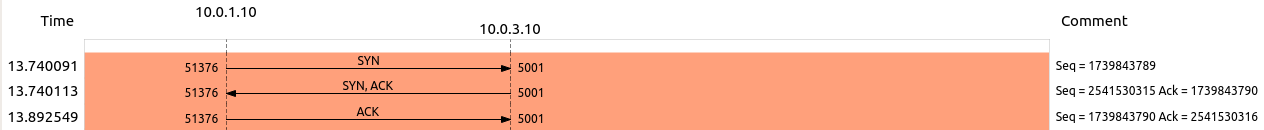
\includegraphics[width=0.95\textwidth]{3-ways-handshake.png}
    \caption{3 Ways Handshake.}
    \label{3-ways-handshake}
\end{figure}

\newpage

\section{Ejercicio 6}

\textit{Qué opciones se negocian. Qué significa c/u? Cuál es el MTU negociado?} \\

Las opciones que se negocian son las siguientes:

\begin{itemize}
    \item \textbf{Maximun Segment Size: 1460 bytes} \\

    El \textbf{Tamaño de segmento máximo} se utiliza para definir el segmento máximo que se utilizará durante una conexión entre dos hosts. 
    Como tal, solo debería ver esta opción utilizada durante la fase SYN y SYN / ACK del handshake de 3 vías. La opción MSS TCP 
    ocupa 4 bytes (32 bits) de longitud. Si ha encontrado anteriormente el término \textit{MTU} que significa Unidad de transferencia 
    máxima, le complacerá saber que el MSS ayuda a definir la MTU utilizada en la red. \\
    
    También nos beneficiaría reconocer la terminología correcta que corresponde a cada nivel del modelo OSI: el encabezado y los 
    datos de TCP se denominan segmento (capa 4), mientras que el encabezado y el segmento de IP se denominan datagramas de IP (capa 3). 
    Además, independientemente del tamaño que tendrá la MTU, la capa Datalink tiene una sobrecarga adicional de 18 bytes. 
    Esta sobrecarga incluye la dirección MAC de origen y destino, el tipo de protocolo, seguido de la secuencia de verificación de 
    trama colocada al final de la trama. \\

    Esta es también la razón por la que solo podemos tener un MTU máximo de 1500 bytes. Como el tamaño máximo de una trama de 
    Ethernet II es de 1518 bytes, restar 18 bytes (sobrecarga de enlace de datos) nos deja con 1500 bytes para jugar. Por lo general, 
    TCP calcula el Tamaño de segmento máximo (MSS) que da como resultado los Datagramas IP que coinciden con la MTU de la red. 
    En la práctica, esto significa que el MSS tendrá un valor tal que, si agregamos también el encabezado IP, el datagrama IP 
    (encabezado IP + encabezado TCP + DATOS) sería igual al MTU de la red. \\

    Si la opción MSS se omite en uno o ambos extremos de la conexión, se utilizará el valor de 536 bytes. El valor MSS de 536 
    bytes está definido por RFC 1122 y se calcula tomando el valor predeterminado de un Datagrama IP, 576 bytes, menos la 
    longitud estándar de la cabecera IP y TCP (40 bytes), que nos da 536 bytes. En general, es muy importante utilizar el mejor 
    valor de MSS posible para su red, ya que el rendimiento de su red podría ser extremadamente bajo si este valor es 
    demasiado grande o demasiado pequeño. \\

    \item \textbf{Sack permited} \\

    \textbf{Selective Acknowledgments}.
    
    TCP ha sido diseñado para ser un protocolo bastante robusto, sin embargo, a pesar de esto, todavía tiene varias 
    desventajas, una de las cuales se refiere a los Reconocimientos, que también es la razón por la que se introdujo 
    el Reconocimiento Selectivo con RFC 1072. El problema con los reconocimientos tradicionales es que no hay 
    mecanismos para que un receptor diga "Todavía estoy esperando los bytes del 20 al 25, pero he recibido los bytes del 30 al 35". 
    Y si se pregunta si esto es posible, entonces la respuesta es "sí", ¡lo es!. Si los segmentos llegan fuera de orden y 
    hay un agujero en la cola del receptor, al usar los Reconocimientos "clásicos" admitidos por TCP, solo se puede decir 
    "He recibido todo hasta el byte 20". El remitente debe reconocer que algo salió mal y continuar enviando desde ese 
    punto en adelante (byte 20). \\

    \item \textbf{Timestamps: TSval 245971, TSecr 245952} \\

    Otro aspecto de los servicios de confiabilidad y control de flujo de TCP son los tiempos de entrega de ida y vuelta que 
    está experimentando un circuito virtual. El tiempo de entrega de ida y vuelta determinará con precisión cuánto tiempo 
    esperará TCP antes de intentar retransmitir un segmento que no se ha reconocido. Debido a que cada red tiene características 
    de latencia únicas, TCP debe comprender estas características para establecer valores de umbral de temporizador de acuse de recibo precisos. \\ 
    
    Las LAN suelen tener tiempos de latencia muy bajos y, como tal, TCP puede usar valores bajos para los temporizadores de confirmación. 
    Si un segmento no se reconoce rápidamente, un remitente puede retransmitir los datos cuestionables rápidamente, minimizando 
    así cualquier pérdida de ancho de banda y retraso. \\
    
    Por otro lado, el uso de un valor de umbral bajo en una WAN seguramente causará problemas simplemente porque los temporizadores 
    de confirmación caducarán antes de que los datos lleguen al destino. Por lo tanto, para que TCP establezca con precisión el valor 
    del umbral del temporizador para un circuito virtual, tiene que medir los tiempos de entrega de ida y vuelta para varios segmentos. 
    Finalmente, debe monitorear segmentos adicionales a lo largo de la vida útil de la conexión para mantenerse al día con los cambios 
    en la red. Aquí es donde la opción de marca de tiempo entra en la imagen. De manera similar a la mayoría de las otras opciones de 
    TCP aquí cubiertas, la opción de marca de tiempo debe enviarse durante el protocolo de enlace de 3 vías para permitir su uso durante 
    cualquier segmento posterior.  \\

    El campo Timestamp consta de un campo Timestamp Echo y Timestamp Reply, los cuales el remitente siempre pone a cero el campo de 
    respuesta y el receptor lo completa, luego de lo cual se envía de vuelta al remitente original. \\

    \item \textbf{No-Operation (NOP)} \\

    La opción nop TCP significa "Sin opción" y se utiliza para separar las diferentes opciones utilizadas dentro del campo Opción TCP. 
    La implementación del campo nop depende del sistema operativo utilizado. Por ejemplo, si se usan las opciones MSS y SACK, 
    Windows XP usualmente colocará dos nop entre ellas. \\
    
    Por último, debemos tener en cuenta que la opción nop ocupa 1 byte. En nuestro ejemplo al principio de la página, ocuparía 
    2 bytes ya que se usa dos veces. También debe tener en cuenta que los hackers suelen comprobar este campo cuando intentan 
    determinar el sistema operativo del host remoto. La opción nop TCP significa "Sin opción" y se utiliza para separar las 
    diferentes opciones utilizadas dentro del campo Opción TCP. La implementación del campo nop depende del sistema operativo utilizado. 
    Por ejemplo, si se usan las opciones MSS y SACK, Windows XP usualmente colocará dos nop entre ellas. Por último, debemos tener en 
    cuenta que la opción nop ocupa 1 byte. En nuestro ejemplo al principio de la página, ocuparía 2 bytes ya que se usa dos veces. También 
    debe tener en cuenta que los hackers suelen comprobar este campo cuando intentan determinar el sistema operativo del host remoto. \\

    \item \textbf{Window scale: 4} \\

    La Windows Scale se define en RFC 1072, que permite que un sistema anuncie valores de tamaño de ventana de 30 bits 
    (16 de la ventana original + 14 de las opciones de TCP), con un tamaño máximo de búfer de 1 GB. Esta opción se ha aclarado 
    y redefinido en RFC 1323, que es la especificación que emplean todas las implementaciones en la actualidad.
\end{itemize}

Luego, como se menciona anteriormente, podemos obtener la MTU sabiendo que,
MTU = IP Header length + TCP Header Length + Data length, [bytes]. \\

En este caso el tamaño del encabezado IP es 20 bytes, el tamaño del encabezado TCP es 40 bytes y el MSS es 1460 bytes, 
por lo tanto $MTU = 20 bytes + 40 bytes + 1460 bytes = 1520 bytes$.

\section{Ejercicio 7}

\textit{Quién es el que envía la mayor cantidad de datos (IP:port)?} \\

El host que envía la mayor cantidad de datos es el cliente, es decir, el host de IP 10.0.1.10.

\newpage

\section{Ejercicio 8}

\textit{Identificar primer segmento de datos (origen, destino, tiempo, número de fila y número de secuencia TCP).} \\

origen: 10.0.1.10, destino: 10.0.3.10, tiempo: 13.892556, fila: 10, número de secuencia: 1739843790.

\begin{figure}[H]
    \centering
    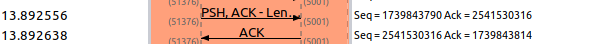
\includegraphics[width=0.95\textwidth]{push.png}
    \caption{Push.}
    \label{push}
\end{figure}

\begin{enumerate}[a)]
    \item Cuántos datos lleva?

    Envía datos de 24bytes.

    \item Cúando es confirmado (tiempo, número de fila y número de secuencia TCP)?

    Podemos ver que en el segmento de tiempo 13.892638, fila 11 y número de secuencia 2541530316,
    se confirman los datos.

    \item La confirmación, qué cantidad de bytes confirma?

    Se confirman 24bytes, y esto lo sabemos por el valor enviado junto al flag ACK, siendo este el numero de secuencia
    del segmento anterior (1739843790) + la cantidad de bytes confirmados.
\end{enumerate}

\section{Ejercicio 9}

\textit{Control de Flujo:}

\begin{enumerate}[a)]
    \item Se activa en algún momento el mecanismo de control de lujo?

    Si, se activa. En los siguientes incisos se explica como y porque.
   
    \item Indicar donde (tiempo, número de fila y número de secuencia TCP) y a que se debe?

    Se activa desde el inicio de la conexión TCP, en el segmento de origen: 10.0.1.10, destino: 10.0.3.10, tiempo: 13.892556, fila: 10, número de secuencia: 1739843790, y esto
    se debe a que es una caracteristica propia del protocolo que permite que no se sobrecargue al receptor con mas bytes de los que puede aceptar.    

    \item Cuánto tiempo parece durar?

    Permanece activo durante toda la conexión TCP, es decir, desde el segmento con numero de fila 9 hasta el segmento
    con numero de fila 1265.

    \item Cuál es el numero de ventana que desactiva el mismo?

    Uno no puede desactivar el control de flujo, pues es un mecanismo propio del protocolo TCP. Sin embargo, cuando el numero de ventana es 0, en ese caso se "desactiva" 
    el control de flujo ya que no se pueden transmitir paquetes al receptor dado que este no puede recibirlos en su buffer.

    \item Qué otros datos se pueden obtener?

    Otro dato que podemos ver es como evoluciona el tamaño de la ventana a lo largo del tiempo.

    El gráfico indica qué tan bien el receptor puede manejar los datos recibidos. Una "línea plana" significa que el receptor no ajustó el tamaño de la ventana, 
    por lo tanto, no tuvo ningún problema para manejar los bytes entrantes lo suficientemente rápido. Un gráfico 'oscilante' significa: el receptor anunciaba un 
    tamaño de ventana más pequeño, ya que no podía manejar el tráfico entrante lo suficientemente rápido, por lo que el búfer se llenó. Al reducir el tamaño de 
    la ventana, le informa al remitente sobre este hecho. El remitente puede o no tomar acción en ese caso. Sin duda, sería inteligente enviar menos datos a la vez. 
    Sin embargo, a menudo no verá ninguna reacción en los escenarios del mundo real. Depende del sistema operativo y de las aplicaciones en uso. \\

    \begin{figure}[H]
        \centering
        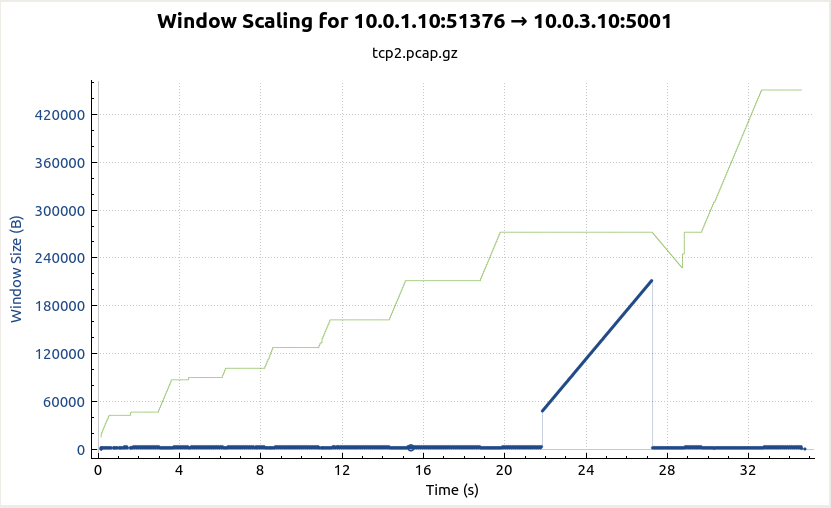
\includegraphics[width=0.65\textwidth]{window.png}
        \caption{Tamaño de la ventana a lo largo del tiempo.}
        \label{window}
    \end{figure}
\end{enumerate}

\section{Ejercicio 10}

\textit{Control de Congestión:}

\begin{enumerate}[a)]
    \item Se encuentra en la red indicios de congestión?

    Si, se encuentran indicios de congestion.

    \item Cómo se detectan?, Indicar un número de segmento perdido.

    En el momento en que uno de los segmentos se pierde, dado que hay mas de 3 segmentos perdidos, es que se produce congestion. Un segmento perdido es
    el segmento con numero de fila 752.

    \item En que momento se ve la primera retransmisión (tiempo y número en el analizador)?

    A partir del paquete 988, time 41.147415 se empiezan a dar las retransmisiones correspondientes a los segmentos.

    \item Cuántos segmentos se re-transmiten?

    Se pueden observar 28 segmentos de retransmisiones.
\end{enumerate}

\section{Ejercicio 11}

\textit{Quién inicia el cierre de la conexión? Qué flags se utilizan? En que segmentos se ve esta (tiempo, número de fila y número de secuencia TCP) ?} \\

Es el host cliente quien inicia el cierre de la conexión. Para esto envia un segmento TCP con el flag FIN activado. Esto se puede ver en el 
segmento de tiempo 48.330648, número de secuencia 1740891638 y número de fila 1263. \\

Cabe destacar que los flags enviados en el segmento son el flag FIN, PSH y ACK, pero solo el flag FIN nos indica el pedido de cierre de conexión. \\

\newpage

\section{Ejercicio 12}

\textit{El RTT entre que valores oscila?} \\

El Round Trip Time (ó RTT) toma valores con una cota mínima de 0 ms y un máximo de 155 ms. Podemos observarlo en la figura (\ref{rtt}). \\

\begin{figure}[H]
    \centering
    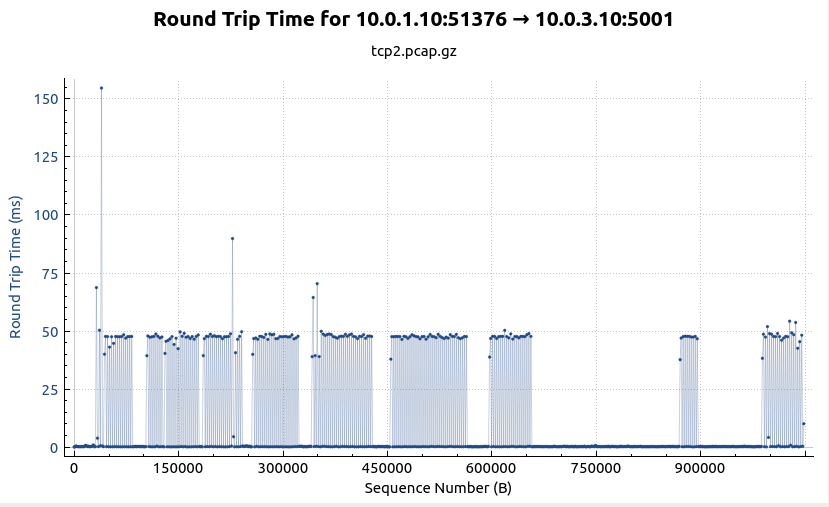
\includegraphics[width=0.65\textwidth]{rtt.png}
    \caption{Round Trip Time.}
    \label{rtt}
\end{figure}

\section{Ejercicio 13}

\textit{El BW digital alcanzado, cual parece ser?} \\

En la figura (\ref{bw}) se puede observar que el BW digital alcanzado es de $270000 \frac{bits}{s}$.

\begin{figure}[H]
    \centering
    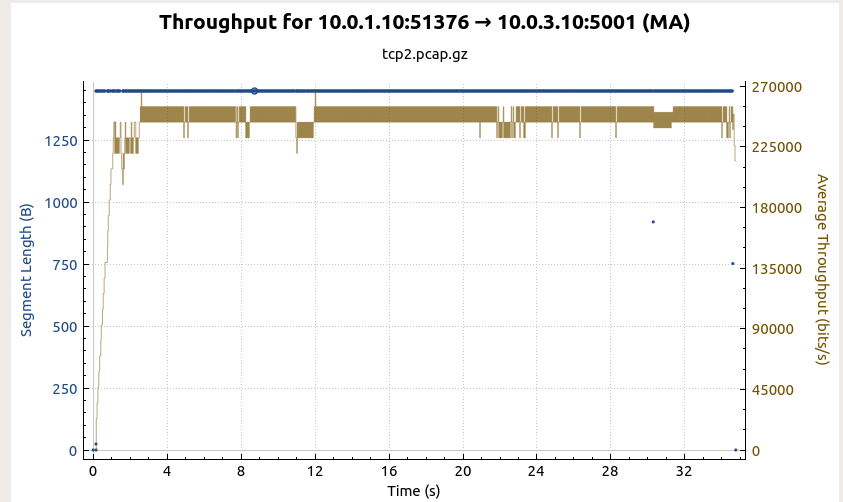
\includegraphics[width=0.65\textwidth]{bw.png}
    \caption{Ancho de banda.}
    \label{bw}
\end{figure}

\newpage

\section{Ejercicio 14}

\textit{Qué otros datos puede obtener de la captura sobre el flujo analizado?} \\

Otros datos que se pueden obtener son los siguientes: \\

Por un lado tenemos el gráfico de \textbf{Time Sequence (Stevens)}. Este es un gráfico 
simple que permite ver la evolución del número de secuencia TCP a lo largo del tiempo, 
similar a los utilizados en la serie de libros "Ilustrados TCP / IP" de Richard Stevens. \\

\begin{figure}[H]
    \centering
    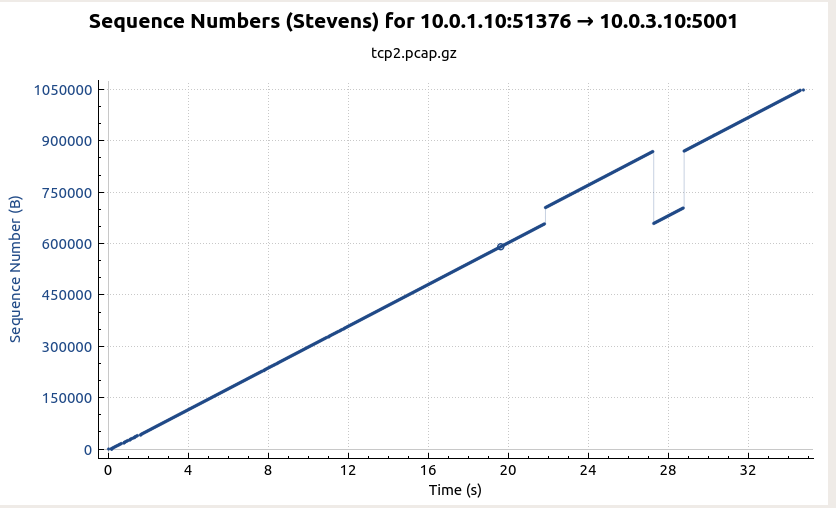
\includegraphics[width=0.65\textwidth]{stevens.png}
    \caption{Gráfico de Número de secuencia TCP vs tiempo utilizando stevens.}
    \label{stevens}
\end{figure}

Por otro lado tenemos la gráfica de \textbf{Time Sequence (tcptrace)}. Este gráfico muestra métricas de TCP 
similares a la utilidad tcptrace, que incluyen segmentos hacia adelante, acuses de recibo, 
acuses de recibo selectivos, tamaños de ventana inversa y cero ventanas. \\

\begin{figure}[H]
    \centering
    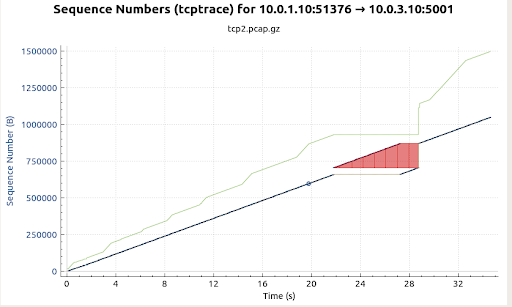
\includegraphics[width=0.65\textwidth]{tcptrace.png}
    \caption{Gráfico de Número de secuencia TCP vs tiempo utilizando tcptrace.}
    \label{tcptrace}
\end{figure}

\end{document}
